\section{Auswertung}
\label{sec:Auswertung}

\subsection{Magnetfeld einer kurzen und einer langen Spule}

Für das Magnetfeld einer Spule der Länge $l=\SI{0,16}{m}$ mit $n=300$ Windungen,
die von einem Strom $I=\SI{1,4}{A}$ durchflossen wird, ergeben sich die in
\ref{fig:lange_spule} dargestellten Messwerte. Die zugrundeliegenden Daten können
\ref{tab:einzelne_spulen} entnommen werden. Der Theoriewert wird nach \ref{eqn:spuleungenaehert} berechnet.
Der Ursprung wurde dabei an den linken Rand der Spule gelegt, wobei berücksichtigt werden
muss, dass die Windungen erst $1,5$cm weiter begonnen.

\begin{figure}
  \centering
  \includegraphics{build/lange_spule.pdf}
  \caption{Auftragung der Messwerte für die magnetische Feldstärke $B$ der langen Spule
  in Abhängigkeit der Position $r$ auf der Achse}
  \label{fig:lange_spule}
\end{figure}

Auffällig ist, dass der theoretisch zu erwartenede Maximalwert mit $B_{\symup{theo}}=3,20$\,mT
zunächst sehr weit über dem gemessenen Wert liegt. Da in der Theorie die magnetische
Feldstärke für große Abstände gegen Null geht, kann jedoch der Wert, dem sich die
Messwerte annähern, als Nullnievau angenommen und von dem theoretischen Erwartungswert
subtrahiert werden, sodass sich für den theoretisch zu erwartenden Maximalwert nun
$B_{\symup{theo}}=2,57$\,mT ergibt. Dabei entspricht der kleinste genessene Wert für die Feldstärke
in guter Näherung dem Nullniveau.

Es ist erkennbar, dass die Messwerte grundlegend dem theoretisch erwarteten Verlauf folgen.
Im Spuleninneren sind sie annähernd konstant und bleiben nur leicht hinter dem
theoretischen Erwartungswert zurück. Der Verlauf zeigt zudem ein starkes Abfallen
der magnetischen Feldstärke am Rand der Spule. Für große Abstände $r$ geht die magnetische
Feldstärke gegen einen konstanten Wert, der jedoch nicht dem theoretisch erwarteten
Wert $B=0$\,mT entspricht. Außerdem ist der Verlauf der Messwerte nicht komplett symmetrisch,
wie es theoretisch zu erwarten wäre.


Für das Magnetfeld einer kurzen Spule mit $l=\SI{0,055}{m}$ Länge und $n=100$ Windungen,
die von einem Strom $I=\SI{1,2}{A}$ durchflossen wird, ergeben sich die Messwerte, die in
\ref{fig:kurze_spule} dargestellt sind. Die Messwerte können \ref{tab:einzelne_spulen}
entnommen werden. Dabei wurden an den Stellen, die mit einem Strich markiert sind keine
Werte augenommen.
Der Theoriewert für die kurze Spule wird ebenfalls mit \ref{eqn:spuleungenaehert} berechnet.

\begin{figure}
  \centering
  \includegraphics{build/kurze_spule.pdf}
  \caption{Auftragung der Messwerte für die magnetische Feldstärke $B$ der kurzen Spule
  in Abhängigkeit der Position $r$ auf der Achse}
  \label{fig:kurze_spule}
\end{figure}


Auch hier ist der Theoretische Erwartungswert mit $B_{\symup{theo}}=2,33$\,mT zunächst
weit über dem Messwert. Nimmt man jedoch den kleinsten gemessenen Wert als Nullniveau
an und subtrahiert diesen Wert von dem theoretischen Erwartungswert, so ergibt sich
$B_{\symup{theo}}=1,76$mT, was sehr nah an den gemessenen Werten liegt.

Der Verlauf der Messwerte für die magentische Feldstärke zeigt auch hier grundlegend
den theoretisch erwarteten Verlauf, allerdings leicht verschoben. Wie bei einer kurzen Spule auch theoretisch
zu erwarten ist, ist das Feld auch im Inneren nicht konstant und fällt an den Rändern
schnell ab. Erneut geht hier die magnetische Feldstärke für große Abstände $r$ nicht
gegen Null, sondern gegen den konstanten Wert $B=-0,57$\,mT.


\begin{table}
  \centering
    \caption{Messdaten zum Magnetfeld der langen Spule $B_{\symup{l}}$ und der
    kurzen Spule $B_{\symup{k}}$}
    \label{tab:einzelne_spulen}
    \begin{tabular}{c c c}
      \toprule
      $r$/cm & $B_{\symup{l}}/$mT & $B_{\symup{k}}/$mT\\
      \midrule
      -9	&  -0,63 &	  -0,56\\
      -8	&  -0,63 &	  -0,56\\
      -7	&  -0,62 &	  -0,56\\
      -6	&  -0,65 &	  -0,55\\
      -5	&  -0,62 &	  -0,53\\
      -4	&  -0,57 &	  -0,51\\
      -3	&  -0,53 &  -0,46\\
      -2	&  -0,45 &  -0,38\\
      -1	&  -0,24 &   -0,24\\
      0	  &  0,04 &    0,06\\
      1	  &  0,65 &   0,65\\
      2	  &  1,50 &   1,28\\
      3	  &  2,01 &   1,68\\
      4	  &  2,28 &   1,77\\
      5	  &  2,37 &   1,59\\
      6   &  2,40 &   1,13\\
      7	  &  2,41 &   0,47\\
      8	  &  2,42 &  -0,02\\
      9	  &  2,41 &  -0,31\\
      10	&  2,40  &  -0,42\\
      11	&  2,38  &  -0,49\\
      12	&  2,35  &  -0,51\\
      13	&  2,29  &  -0,53\\
      14	&  2,20  &  -0,54\\
      15	&  2,05  &  -0,55\\
      16	&  1,69  &  -0,56\\
      17	&  1,02  &  -0,56\\
      18  &  0,24  &  -0,57\\
      19	&  -0,20 & -\\
      20	&  -0,17 & -\\
      21	&  -0,32 & -\\
      22	&  -0,43 & -\\
      23	&  -0,48 & -\\
      24	&  -0,52 & -\\
      25	&  -0,53 & -\\
      26	&  -0,54 & -\\
      27	&  -0,55 & -\\
      28	&  -0,55 & -\\
      \bottomrule
    \end{tabular}
\end{table}

\newpage
\subsection{Magnetfeld eines Helmholtzspulenpaares}

Nun soll die magnetische Feldstärke eines Helmholtzspulenpaares in Abhängigkeit von
der Posistion auf der durch die Spulenmittelpunkte verlaufenden Achse bestimmt werden.
Wird ein Spulenpaar mit je $n=100$ Windungen und einem Durchmesser $D=0,125$\,m
von einem Strom $I=5$\,A durchflossen, so ergeben sich die Messwerte aus \ref{tab:helmholtz}
und \ref{tab:helmholtz_f}.
Dabei entspricht der Abstand der beiden Spulen voneinander ihrem Radius.
Der theoretisch maximal zu erwartende Wert ergibt sich gemäß \ref{eqn:helmholz} zu $B_{\symup{theo}}=7,19$\,mT. In
\ref{fig:spulenpaar_5} sind die Messwerte, sowie die Theoriekurve graphisch dargestellt. Der Ursprung wurde
dabei in das Zentrum zwischen beiden Spulen gelegt. Es sei hierbei darauf
hingewiesen, dass zwischen beiden Spulen nur in einem sehr kleinen Bereich Messwerte
aufgenommen werden konnten, da die verwendeten Spulen selbst recht breit waren.

\begin{figure}
  \centering
  \includegraphics{build/spulenpaar_5.pdf}
  \caption{Auftragung der Messwerte für die magnetische Feldstärke $B$ des Helmholtzspulenpaares
  in Abhängigkeit der Position $r$ auf der Achse für $I=5$\,A}
  \label{fig:spulenpaar_5}
\end{figure}

Es ist erkennbar, dass die Messwerte zwischen den Spulen nur minimal hinter dem theoretischen Erwartungswert
zurückbleiben. Die Messwerte außerhalb des Spulenpaares fallen exponentiell und gehen
wie theoretisch zu erwarten ist gegen null. Jedoch lassen sich anhand der Messung keine
genauen Aussagen über das Verhalten des Feldes in einer der beiden Spulen treffen.
Da die Messwerte insgesamt jedoch sehr gut den Verlauf der Theoriekurve widerspiegeln,
kann angenommen werden, dass die Theoriekurve das reale Feld auch in diesem Bereich gut beschreibt.


Die Messung wird für einen Strom von $I=3$\,A wiederholt. Die aufgenommenen Messwerte
befinden sich ebenfalls in \ref{tab:helmholtz} und \ref{tab:helmholtz_f}. Der theoretisch maximal zu
erwartende Wert ergibt sich hier ebenfalls nach \ref{eqn:helmholz} zu $B_{\symup{theo}}=4,32$\,mT. Die Messwerte
und die Theoriekurve sind in \ref{fig:spulenpaar_3} dargestellt. Hier wurde der Ursprung ebenfalls genau
zwischen die beiden Spulen gelegt.

\begin{figure}
  \centering
  \includegraphics{build/spulenpaar_3.pdf}
  \caption{Auftragung der Messwerte für die magnetische Feldstärke $B$ des Helmholtzspulenpaares
  in Abhängigkeit der Position $r$ auf der Achse für $I=3$\,A}
  \label{fig:spulenpaar_3}
\end{figure}

Hier liegen die Messwerte zwischen den beiden Spulen deutlich unter dem
theoretische Erwartungswert. Außerhalb der Spulen zeigt sich jedoch erneut ein
exponentieller Abfall der Messwerte für die magentische Feldstärke, wobei diese für
große Abstände $r$ gegen null gehen.


\begin{table}
  \centering
  \caption{Messdaten zum Magnetfeld des Helmholtzspulenpaares bei 5A ($B_{\symup{1}}$)
  und 3A ($B_{\symup{2}}$)}
  \label{tab:helmholtz}
  \begin{tabular}{c c c}
    \toprule
    $r/$cm & $B_{\symup{1}}/$mT & $B_{\symup{2}}/$mT\\
    \midrule
    -0,5	&  7,077 & 4,161\\
    -0,4	&  7,088 & 4,164\\
    -0,3	&  7,092 & 4,167\\
    -0,2	&  7,094 & 4,168\\
    -0,1	&  7,097 & 4,169\\
    0	    &  7,097 & 4,170\\
    0,1	  &  7,099 & 4,171\\
    0,2	  &  7,099 & 4,171\\
    0,3	  &  7,099 & 4,171\\
    0,4	  &  7,093 & 4,168\\
    0,5	  &  7,078 & 4,154\\
    6	    &  4,703 & 2,772\\
    6,5	  &  4,301 & 2,530\\
    7	    &  3,936 & 2,301\\
    7,5	  &  3,573 & 2,097\\
    8	    &  3,222 & 1,897\\
    8,5	  &  2,896 & 1,714\\
    9	    &  2,599 & 1,542\\
    9,5 	&  2,325 & 1,392\\
    10	  &  2,090 & 1,254\\
    10,5	&  1,864 & 1,128\\
    11	  &  1,682 & 1,017\\
    11,5	&  1,530 & 0,923\\
    12	  &  1,385 & 0,841\\
    12,5	&  1,252 & 0,770\\
    13	  &  1,135 & 0,702\\
    13,5	&  1,033 & 0,645\\
    14	  &  0,950 & 0,609\\
    14,5	&  0,869 & 0,544\\
    15	  &  0,797 & 0,500\\
    15,5	&  0,736 & 0,464\\
    16	  &  0,677 & 0,428\\
    16,5	&  0,627 & 0,397\\
    17	  &  0,580 & 0,370\\
    17,5	&  0,541 & 0,347\\
    18	  &  0,504 & 0,326\\
    18,5	&  0,472 & 0,307\\
    19	  &  0,443 & 0,288\\
    19,5	&  0,416 & 0,272\\
    20	  &  0,391 & 0,256\\
    20,5	&  0,367 & 0,242\\
    21	  &  0,346 & 0,230\\
    \bottomrule
  \end{tabular}
\end{table}

\begin{table}
  \centering
  \caption{Messdaten zum Magnetfeld des Helmholtzspulenpaares bei 5A ($B_{\symup{1}}$)
  und 3A ($B_{\symup{2}}$)(Fortsetzung)}
  \label{tab:helmholtz_f}
  \begin{tabular}{c c c}
    \toprule
    $r/$cm & $B_{\symup{1}}/$mT & $B_{\symup{2}}/$mT\\
    \midrule
    21,5	&  0,328 & 0,219\\
    22	  &  0,311 & 0,210\\
    22,5	&  0,296 & 0,199\\
    23	  &  0,278 & 0,190\\
    23,5	&  0,266 & 0,181\\
    \bottomrule
  \end{tabular}
\end{table}


\newpage
\subsection{Bestimmung der Hysteresekurve einer Toroidspule mit Eisenkern}

Zur Bestimmung der Hysteresekurve der gegebenen mit einem ferromagnetischen Stoff
gefüllten Toroidspule wird die magentische Feldstärke $B$ gegen die Stromstärke
$I$ aufgetragen. Es ergibt sich die Graphik aus \ref{fig:hysterese}. Die gemessenen
Daten können \ref{tab:hysterese} und \ref{tab:hysterese_f}  entnommen werden.

\begin{figure}
  \centering
  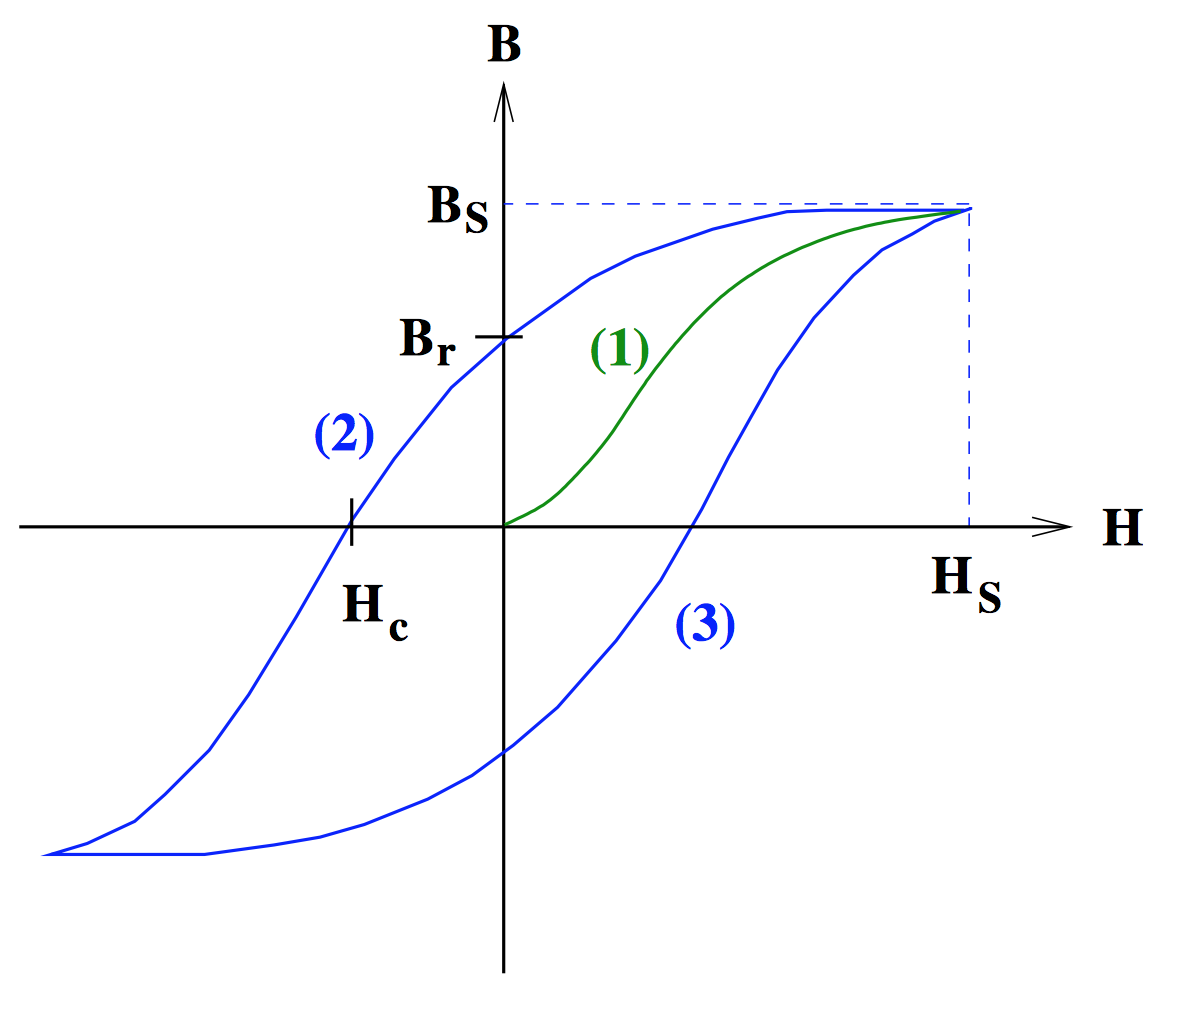
\includegraphics{build/hysterese.pdf}
  \caption{Auftragung der Messwerte für die magnetische Feldstärke der Toroidspule
  in Abhängigkeit von der Stromstärke}
  \label{fig:hysterese}
\end{figure}

\begin{figure}
  \centering
  \includegraphics{build/koerzitiv.pdf}
  \caption{Geraden, aus denen die Stromstärke für die Koerzitivfeldstärke bestimmt werden}
  \label{fig:koerzitiv}
\end{figure}


<<<<<<< HEAD
Für die Remanenz sind die Werte $B_{\symup{r}} = 128,8$mT und $B_{\symup{r}}=-126,1$mT
ablesbar. Da im Bereich um $I=0$ ein annähernd linearer Zusammenhang vorliegt, lässt
||||||| merged common ancestors
Für die Remanenz sind die Werte $B_{\symup{r}}=128,8$mT und $B_{\symup{r}}=-126,1$mT
ablesbar. Da im Bereich um $I=0$ ein annähernd linearer Zusammenhang vorliegt, lässt
=======
Für die Remanenz sind die Werte $B_{\symup{r}}=128,8$\,mT und $B_{\symup{r}}=-126,1$\,mT
ablesbar. Da im Bereich um $I=0$\,A ein annähernd linearer Zusammenhang vorliegt, lässt
>>>>>>> korrigierte einheiten
sich der Strom, bei dem die Koerzitivfeldstärke vorliegt, berechnen, indem aus den vorhandenen
Messwerten Geradengleichungen der Form
\begin{equation}
  f(x)=mx+b
  \end{equation}
aufgestellt werden. Dabei ist $m$ die Steigung der Geraden und $b$ der y-Achsenabschnitt.
Es ergeben sich die Geradengleichungen
\begin{align}
  B_{\symup{1}}(I)&=193,76I+128,8 & B_{\symup{2}}(I)&=191,1I-126,1\,.
\end{align}
Diese sind in \ref{fig:koerzitiv} dargestellt. Dabei besitzt die Steigung die Einheit
T/A.
Bestimmt man deren Nullstellen, so ergeben sich daraus für die Stromstärken, bei
denen die Koerzitivfeldstärke auftritt folgende Werte:
\begin{align}
  I_{\symup{1}}&=-0,665\,\text{A} & I_{\symup{2}}&=0,660\,\text{A}\,.
\end{align}


Der grundlegende Verlauf der Hysteresekurve stimmt mit dem der in \ref{fig:hysteresetheorie}
dargestellten Theoriekurve gut überein, jedoch weist
die gemessene Hysteresekurve nur eine relativ schwache Sättigung auf. Im Idealfall sollte
hier die Steigung gegen null gehen. Insgesamt fällt die Hysteresekurve sehr schmal aus.

\begin{table}
  \centering
  \caption{Messdaten zur magnetischen Feldstärke in der Toroidspule in Abhängigkeit
  vom Strom}
  \label{tab:hysterese}
  \begin{tabular}{c c}
    \toprule
    $I/$A & $B/$mT\\
    \midrule
    1	  &  125,8\\
    2	  &  292,0\\
    3	  &  406,8\\
    4	  &  482,9\\
    5	  &  538,7\\
    6	  &  580,6\\
    7	  &  615,8\\
    8	  &  647,8\\
    9	  &  675,9\\
    10	&  702,1\\
    9	  &  686,5\\
    8	  &  668,3\\
    7	  &  648,6\\
    6	  &  624,3\\
    5	  &  595,3\\
    4	  &  559,7\\
    3	  &  513,5\\
    2	  &  447,2\\
    1	  &  314,5\\
    0	  &  128,8\\
    -1	&  -64,96\\
    -2	&  -240,4\\
    -3	&  -375,9\\
    -4	&  -468,5\\
    -5	&  -530,3\\
    -6	&  -577,5\\
    -7	&  -615,7\\
    -8	&  -648,2\\
    -9	&  -676,5\\
    -10	&  -701,4\\
    -9	&  -686,1\\
    -8	&  -668,2\\
    -7	&  -647,8\\
    -6	&  -624,0\\
    -5	&  -595,5\\
    -4	&  -560,0\\
    -3	&  -513,7\\
    -2	&  -448,2\\
    -1	&  -314,5\\
    0	  &  -126,1\\
    1	  &  65±0,5\\
    2	  &  240,3\\
    \bottomrule
  \end{tabular}
\end{table}

\begin{table}
  \centering
  \caption{Messdaten zur magnetischen Feldstärke in der Toroidspule in Abhängigkeit
  vom Strom(Fortsetzung)}
  \label{tab:hysterese_f}
  \begin{tabular}{c c}
    \toprule
    $I/$A & $B/$mT\\
    \midrule
    3	  &  378,4\\
    4	  &  469,7\\
    5	  &  531,4\\
    6	  &  578,6\\
    7	  &  616,3\\
    8	  &  646,9\\
    9	  &  675,3\\
    10	&  703,6\\
    \bottomrule
  \end{tabular}
\end{table}
